\documentclass[12pt]{article} %Tipo de documento

\usepackage[utf8]{inputenc}	%Codificación
\usepackage[spanish]{babel} %Idioma
\usepackage{fancyhdr, graphicx, parskip}
\usepackage[margin=1in]{geometry} %para el identado de párrafos
\usepackage{indentfirst}%para el identado de párrafos
\usepackage{array}%Tamaño de celdas
\usepackage{blindtext}%Enumeraciones
\usepackage{xcolor}
\usepackage{hyperref} %enlaces
\usepackage{colortbl} %Color de las tablas

\graphicspath{ {images/} } %Para las imagenes del fancyhead
\renewcommand{\headrulewidth}{0pt}
\pagestyle{empty}


\fancyhead[L]{
	
\includegraphics[width=2cm]{unam.jpg}
}
\fancyhead[R]{
	
\includegraphics[width=2cm]{FI.jpg}
}
\fancyfoot[C]{}

\title{Propuesta de proyecto final}
\author{Gabriel Rojas, Max Schouten, Fernanda Jiménez}
\date{\today}

\begin{document}
	%Portada
	\begin{titlepage}
		\thispagestyle{fancy}
		\centering
		{\bfseries - \par}
		\vspace{1cm}
		{\bfseries\LARGE UNIVERSIDAD NACIONAL AUTÓNOMA DE MÉXICO \par}
		\vspace{1cm}
		{\bfseries\LARGE Facultad de Ingeniería \par}
		\vspace{1cm}
		{\bfseries\LARGE Computación Gráfica e Interacción Humano Computadora \par}
		\vspace{1cm}
		{\bfseries\LARGE Ing. Arturo Pérez de la Cruz \par}
		\vspace{1cm}
		{\bfseries\LARGE Propuesta de proyecto final \par}
		\vspace{1cm}
		{\bfseries\LARGE Cruz Schouten Max Bernardo \par}
		{\bfseries\LARGE Jiménez García Fernanda \par}
		{\bfseries\LARGE Rojas Méndez Gabriel \par}
		\vspace{1cm}
		{\bfseries\LARGE Fecha de entrega: 27 de marzo de 2020 \par}
		\vspace{1cm}
		{\bfseries\LARGE Semestre 2020-2 \par}
	\end{titlepage}
	
	
	\newpage
	
	\section{Descripción general}
	
	\setlength{\parindent}{1.0cm}
	Recorrido virtual de un entorno jurásico basado en voxel art, incluyendo elementos que simulen un parque temático. 
	Tendrá dinosaurios, jaulas, vegetación e iluminación para simular el ambiente virtual. 
	Se incluirá una cámara en tercera persona para nuestro avatar y una cámara aérea que será desde el helicóptero.
	\setlength{\parindent}{0.0cm}
	
	\section{Diseño de ambiente virtual}
	
	\begin{figure}[h]
		\begin{center}
			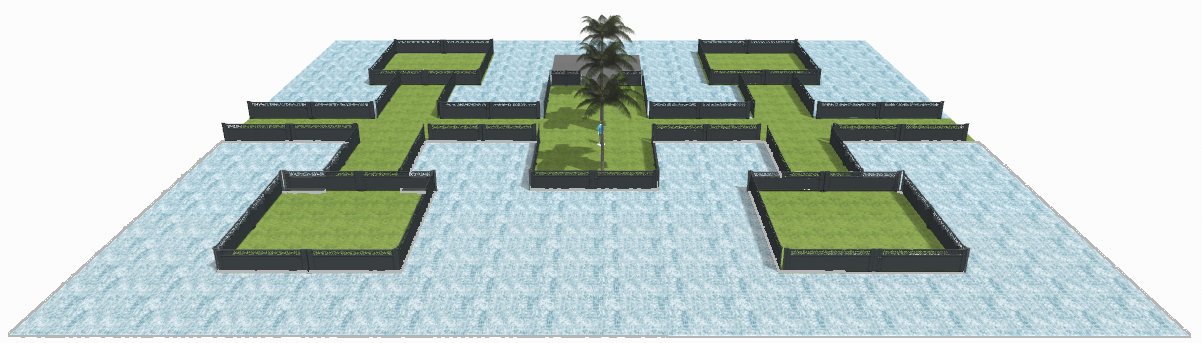
\includegraphics[scale=1.65]{images/vista.png}
			\caption{Islas}
		\end{center}  		
	\end{figure}
	
	\setlength{\parindent}{1.0cm}
	Se propone una distribución de elementos similar a la Figura 1, 4 jaulas circulares, una por cada dinosaurio. 
	Cada dinosaurio estará en una pequeña isla con luces spotlight y vegetación, 
	cada isla estará conectada con caminos de concreto. 
	Los caminos tendrán lámparas que se encenderán dependiendo si es de noche o de día. 
	Cada isla contará con 2 luces spotlight, una de ellas se encenderá y apagará con teclado y la otra servirá para 
	un show de luces que igual será activada mediante teclado.
	\setlength{\parindent}{0.0cm}
	
	\begin{figure}[h]
		\begin{center}
			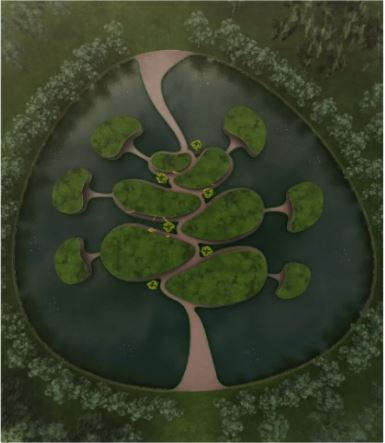
\includegraphics[scale=0.5]{images/Isla.JPG}
		\caption{Referencia de islas}
		\end{center}  		
	\end{figure}
	
	
	\newpage
	
	\section{Modelos a utilizar}
	
	\begin{center}
		\begin{tabular}{ | m{19em} | m{19em} | }
			\hline
			\rowcolor[rgb]{0.6,0.8,1.0}
			\textbf{Nombre} & \textbf{Animación}  \\ 
			\hline
			\hline
			\rowcolor[rgb]{0.4,0.6,1.0}
		 	Tiranosaurio rex &
		 	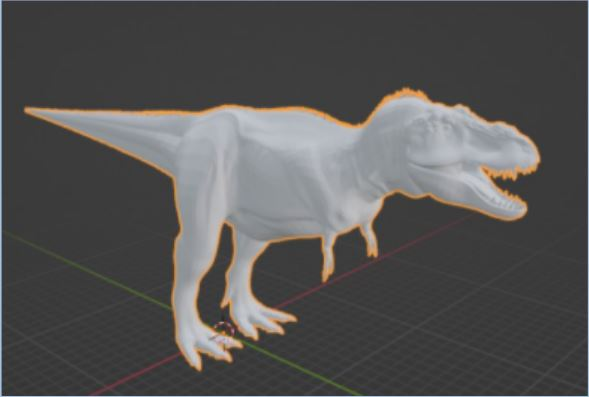
\includegraphics[scale=0.5]{images/Tiranosaurio.JPG} \\  
		 	\hline
		 	\rowcolor[rgb]{0.6,0.8,1.0}
		 	Cuello largo (Diplodocus) &
		 	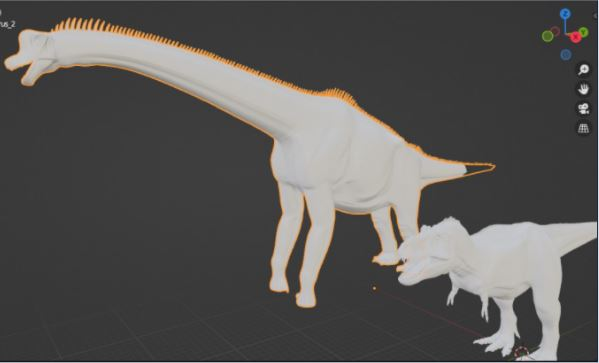
\includegraphics[scale=0.5]{images/Diplodocus.JPG} \\
		 	\hline
		 	\rowcolor[rgb]{0.4,0.6,1.0}
		 	Estegosaurio &
		 	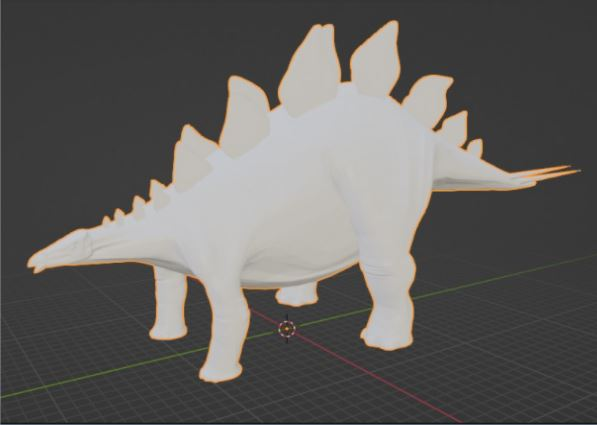
\includegraphics[scale=0.5]{images/Estegosaurio.JPG} \\  
			\hline
		\end{tabular}
	\end{center}
	\begin{center}
		\begin{tabular}{ | m{19em} | m{19em} | }
			\hline
			\rowcolor[rgb]{0.6,0.8,1.0}
			\textbf{Nombre} & \textbf{Animación}  \\  
		 	\hline
		 	\hline
		 	\rowcolor[rgb]{0.4,0.6,1.0}
		 	Velociraptor &
		 	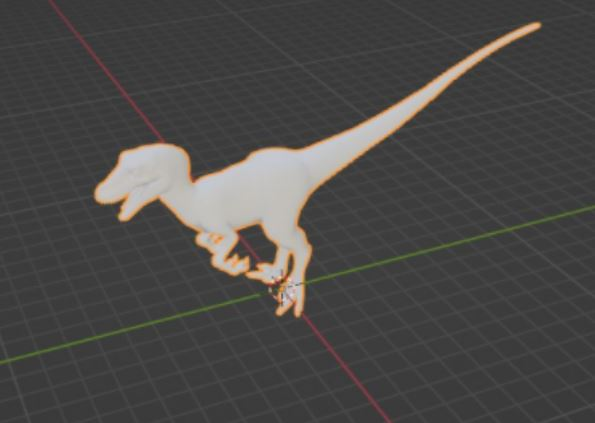
\includegraphics[scale=0.5]{images/Velociraptor.JPG} \\  
		 	\hline
		 	\rowcolor[rgb]{0.6,0.8,1.0}
		 	Helicóptero &
		 	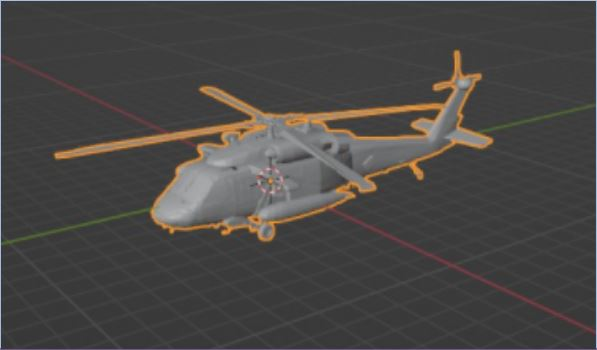
\includegraphics[scale=0.5]{images/Helicoptero.JPG} \\  
			\hline
			\rowcolor[rgb]{0.4,0.6,1.0}
		 	Avatar &
		 	
\includegraphics [scale=0.5]{ images/Avatar.JPG} \\  
			\hline
		\end{tabular}
	\end{center}

	%Desarrollo de la introducción.
	\newpage
	
	\section{Texturizado}
	
	\setlength{\parindent}{1.0cm}
	Cada uno de los elementos empleados para la elaboración de este proyecto serán texturizados de tal manera que sean realistas y congruentes, como en el caso de los dinosaurios en donde las texturas se aproximarán a lo más realista que se pueda. En el caso del avatar principal, de igual manera se propone una textura fiel a la apariencia del personaje Bender de la serie animada \textit{Futurama.}
	\setlength{\parindent}{0.0cm}
	
	\section{Elementos diferentes}
	
	\begin{itemize}
		\item[\textbullet] Dinosaurios (4)
		\item[\textbullet] Árboles (2)
		\item[\textbullet] Arbustos (2)
		\item[\textbullet] Pasto (1)
		\item[\textbullet] Agua (1)
		\item[\textbullet] Concreto (1)
		\item[\textbullet] Helicóptero (1)
		\item[\textbullet] Lámparas (1)
		\item[\textbullet] Spotlight (1)
 	\end{itemize}
 	
 	Éstos elementos serán únicos pero podrán repetirse a lo largo del escenario.
 	
 	\section{Animaciones tentativas}
	
	\begin{itemize}
		\item[\textbullet] \emph{Velociraptor:} Correr por el área de su jaula moviendo sus extremidades (piernas), detenerse ver a los lados.
		\item[\textbullet] \emph{Diplodocus:} Ver a su alrededor, asegurándose que no haya presas y después bajarse a comer pasto, 
					o bien comer de un árbol.
		\item[\textbullet] \emph{Tiranosaurio:} Grito en donde se podrá observar que abre la mandibula levanta sus extremidades (brazos) y mueve su cabeza de izquierda a derecha.
		\item[\textbullet] \emph{Estegosaurio:} Caminata por su jaula moviendo sus cuatro extremidades y su cola, se detiene para bajar y subir su cuello.
		\item[\textbullet] \emph{Helicóptero:} Aceleración gradual de hélices, elevación y recorrido determinado del zoológico. 
				Inclinaciones (izquerda, derecha, adelante, atrás) y giro (izquierda, derecha).
		\newpage
		\item[\textbullet] \emph{Avatar:} Caminata tipo Roblox por las jaulas del zoológico.
		\item[\textbullet] \emph{Duración aproximada de las animaciones:} Todas las animaciones tienen una tentativa de entre 5 y 15 segundos.
 	\end{itemize}
 	
 	\section{Cronograma de actividades}
 	
 	\begin{center}
 		\def\arraystretch{1.5} %permite el espaciado dentro de las celdas
		\begin{tabular}{ | m{1.5em} | m{12em} | m{5.5em} | m{5.5em} | m{3em} | m{5.5em} |}
			\hline
			\rowcolor[rgb]{0.6,0.8,1.0}
			\textbf{\#} & \textbf{Actividad} & \textbf{Fech}& \textbf{Horario} & \textbf{Horas} & \textbf{Costo} \\ 
			\hline
			\hline
			\rowcolor[rgb]{0.8,0.6,1.0}
			1 & Planeación de la distribución y diseño del espacio virtual, selección de modelo a emplear & 21/03/2022 & 18:00-20:00 & 2 & 364.4 \\ 
			\hline
			\rowcolor[rgb]{0.6,0.8,1.0}
			2 & Diseño base del ambiente virtual & 23/03/2022 & 18:00-20:00 & 2 & 232.88 \\ 
			\hline
			\rowcolor[rgb]{0.8,0.6,1.0}
			3 & Modelado del ambiente virtual & 23/03/2022 & 18:00-20:00 & 2 & 364.4 \\ 
			\hline
			\rowcolor[rgb]{0.6,0.8,1.0}
			4 & Modelado de los elementos que serán parte del espacio & 26/03/2022 & 18:00-20:00 & 2 & 364.4 \\ 
			\hline
			\rowcolor[rgb]{0.8,0.6,1.0}
			5 & Cámara sintética & 28/03/2022 & 18:00-20:00 & 2 & 364.4\\ 
			\hline
			\rowcolor[rgb]{0.6,0.8,1.0}
			6 & Proyecciones &  30/03/2022 & 18:00-20:00 & 2 & 364.4 \\ 
			\hline
			\rowcolor[rgb]{0.8,0.6,1.0}
			7 & Texturizado & 2/04/2022 & 18:00-23:00 & 5 & 582.2 \\ 
			\hline
			\rowcolor[rgb]{0.6,0.8,1.0}
			8 & Iluminación & 4/04/2022 & 18:00-20:00 & 2 & 232.88 \\ 
			\hline
			\rowcolor[rgb]{0.8,0.6,1.0}
			9 & Animación I & 6/04/2022 & 18:00-20:00 & 2 & 232.88 \\ 
			\hline
			\rowcolor[rgb]{0.6,0.8,1.0}
			10 & Animación II  & 9/04/2022 & 18:00-20:00 & 2 & 232.88 \\ 
			\hline
			\rowcolor[rgb]{0.8,0.6,1.0}
			11 & Animación III & 11/04/2022 & 18:00-20:00 & 2 & 232.88 \\ 
			\hline
			\rowcolor[rgb]{0.6,0.8,1.0}
			12 & Animación IV & 13/04/2022 & 18:00-20:00 & 2 & 232.88 \\ 
			\hline
			\rowcolor[rgb]{0.8,0.6,1.0}
			13 & Animación V & 16/04/2022 & 18:00-20:00 & 2 & 232.88 \\ 
			\hline
			\rowcolor[rgb]{0.6,0.8,1.0}
			14 & Elaboración del Manual de usuario & 18/04/2022 & 18:00-20:00 & 2 & 364.4 \\ 
			\hline
			\rowcolor[rgb]{0.8,0.6,1.0}
			15 & Elaboración del video  & 19/04/2022 & 18:00-19:00 & 1 & 182.2 \\ 
			\hline
			\rowcolor[rgb]{0.6,0.8,1.0}
			16 & Entrega del proyecto & 20/04/2022 & de clase & 0 & sin costo \\ 
			\hline
		\end{tabular}
	\end{center}
	
	\newpage
	\underline{Salario individual total:}
	
	\$4580.96
	
	\underline{Costo final}
	
	\$13,742.88
	
	\underline{Trabajos considerados:}
	
	Dibujante de construcción 
	\color{gray}(116.44 por hora)\color{black}
	, Dibujante de Ingeniería y Arquitectura 
	\color{gray}(116.44 por hora)\color{black}
	, Ingeniero 
	\color{gray}(182.2 por hora)\color{black}	
	
	\section{Sistema de control de versiones}
	\setlength{\parindent}{1.0cm}
	Para una exitoso desarrollo se emplearan herramientas que faciliten la colaboración y comunicación del equipo de trabajo, llevando así un control detallado de las actividades realizadas por cada uno y clara y concisa comunicación que agilice cada uno de los procesos implementados.
	\setlength{\parindent}{0.0cm}
	
	\begin{itemize}
		\item[\textbullet] \emph{\textbf{GitHub:}} con esta herramienta se llevará un control de versiones con respecto a las modificaciones e integraciones que se vayan realizando al código, además de que se facilitará el desarrollo paralelo del proyecto, también se aprovechará la herramienta de GitHub Project la cual permite la creación de tareas y asignación a los colaboradores del repositorio. Para más información se puede visitar el \color{blue}\href{https://github.com/GabooLml/ProyectoFinalCGIHC20222}{\textbf{repositorio}} \color{black}
		\begin{figure}[h]
			\begin{center}
				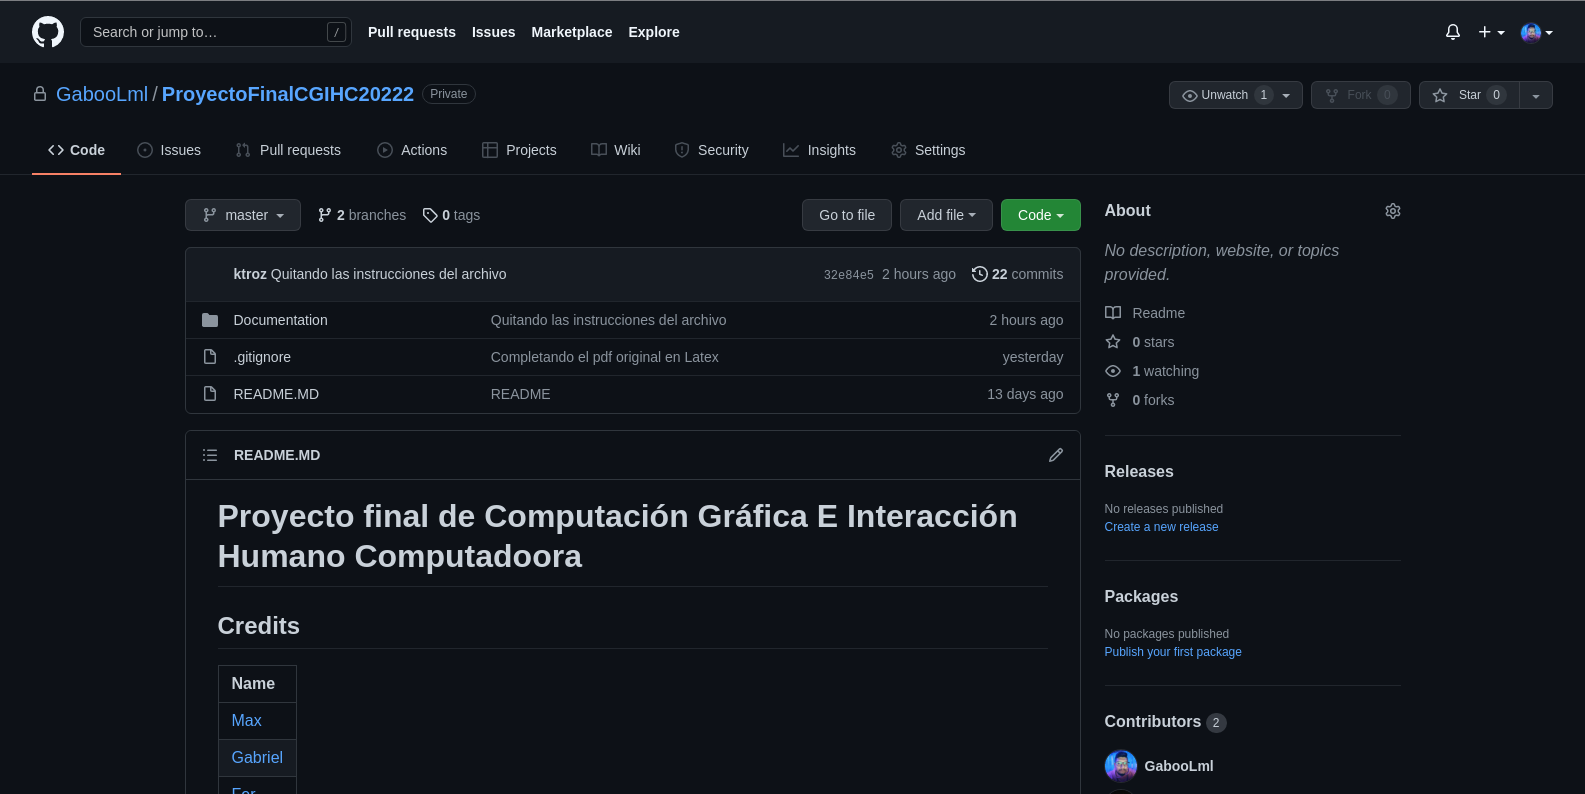
\includegraphics[scale=0.99]{images/repo.png}
				\caption{Repositorio}
			\end{center}  		
		\end{figure}
		
		\newpage
		\item[\textbullet] \emph{\textbf{Google Drive:}} esta herramienta nos permitirá elaborar y documentar información relevante del proyecto como lo son el manual de usuario, manual técnico, documentación en general y diagrama de planificación de actividades (diagrama de Gantt). Toda esta información está disponible en el siguiente enlace. \color{blue}\href{https://drive.google.com/drive/folders/1gjJ3EJFGPzE9q7rekX6cMGJpEYtjIQUh?usp=sharing}{\textbf{Documentación}} \color{black}
		\begin{figure}[h]
			\begin{center}
				\includegraphics[scale=0.99]{images/drive.png}
				\caption{Sistema de archivos compartidos}
			\end{center}  		
		\end{figure}
	
		\item[\textbullet] \emph{\textbf{WhatsApp:}} Para una comunicación informal y más rápida se empleará este sistema de mensajería instantánea, en donde se podrán abordar temas mínimos y rápidos, respecto a reuniones para revisiones de avances o resolución de dudas. 
		\begin{figure}[h]
			\begin{center}
				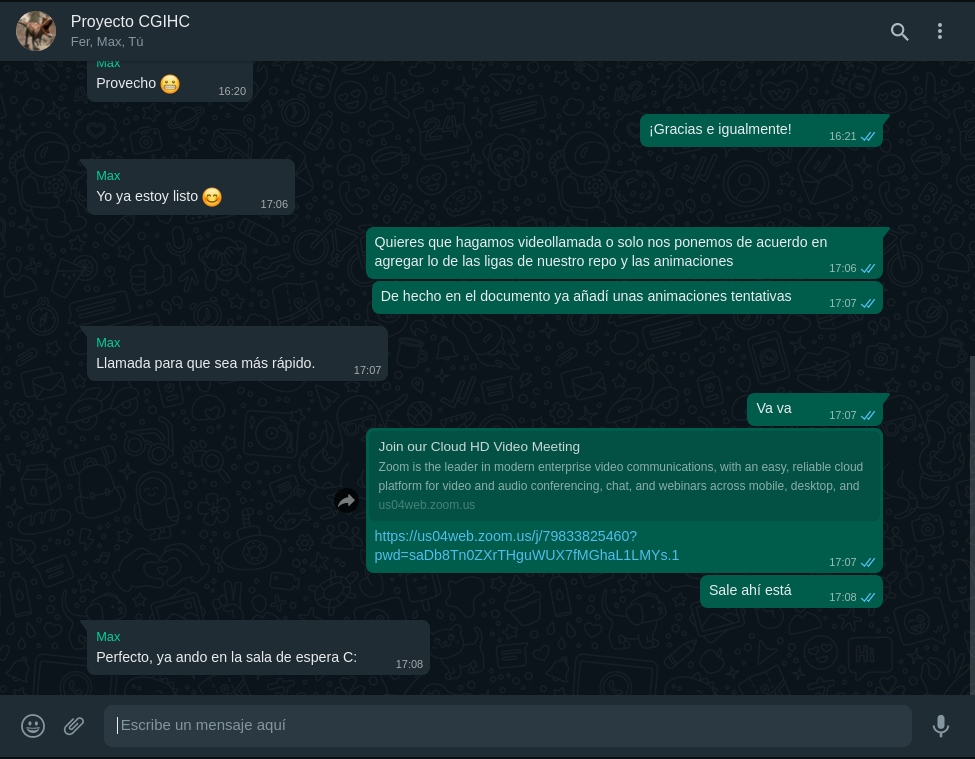
\includegraphics[scale=0.99]{images/grupo.png}
				\caption{Comunicación por mensajería instantánea}
			\end{center}  		
		\end{figure}
\end{itemize}

    \newpage
	\section{Comentarios}
 	
	\emph{Cruz Schouten Max Bernardo:}
	La elaboración de ésta propuesta nos ayudó a tener un panorama general, además de que logramos establecer un escenario 
	base que iremos moldeando a lo largo del proyecto. Por otro lado, nuestro cronograma nos ayudó a dividir el proyecto en 
	tareas más pequeñas, fue interesante ver cómo afectó en el costo final a pesar de contar con modelos con licencia libre.
	\\
	
	\emph{Jiménez García María Fernanda:}
	Para la elaboración de la propuesta se establecieron objetivos generales tanto a largo, como a corto plazo, con la 
	finalidad de dividir el trabajo eficientemente, dando continuidad y cumpliendo con los requerimientos del proyecto. 
	Así mismo, es importante resaltar que durante el proceso de elaboración, se establecerán los objetivos particulares a 
	cada actividad propuesta que estarán sujetos a cambios. Se tiene previsto dedicar 8 horas por semana,  los lunes, 
	miércoles y sábados, se consideró tanto la planeación y el diseño, como la implementación que incluye modelado, 
	texturizado, iluminación y animación, así como documentación. Para cada actividad se estableció un costo por persona, 
	simulando un proyecto laboral. Se consideraron distintos diseños para el ambiente virtual, y la propuesta final nos pareció 
	estética y lo suficientemente compleja para el diseño de un parque jurásico.
	\\
	
	\emph{Rojas Méndez Gabriel:}
	el haber planificado y proyectado lo que queremos desarrollar nos permite determinar tareas más precisas con las cuales 
	buscamos optimizar tiempos en el desarrollo de este proyecto, se tiene previsto que puedan hacerse presentes algunos 
	contratiempos pero que estos no eleven el tiempo de trabajo establecido. Además, con esta planificación se está ejecutando 
	una buena práctica dentro del desarrollo de proyectos, con la cual se pueden dividir las tareas entre los integrantes del 
	equipo de manera más eficiente, ya que al se tiene establecido los resultados que se quieren obtener, otro tema abordado en 
	esta planificación es determinar costos y precio del proyecto, en donde nos basamos a los tabuladores nacionales de salarios, 
	tiempos y nivel de dificultad, y aunque tal vez el precio tenga ciertas variaciones por nuestra falta de experiencia dentro 
	de la temática de los precios esperamos que este sea lo más cercano a lo del mundo laboral.
 	
	\section{Bibliografía}
	
	tlreichen (s.f.) \emph{Modelo de avatar.} ClaraIO. Recuperado el 19/03/2022
	\color{blue}\url{https://clara.io/view/18fd810f-8b42-4ff0-9d4b-0aeb68d445b9}\color{black}
	\\
	
	IMSS-SNTSS. (16/10/2020) \emph{Tabulador de sueldos para personal base.} SNTSS. 
	\color{blue}\url{http://www.sntss.org.mx/filesUpdates/tabulador-de-sueldos.pdf}\color{black}
	
\end{document}	